% === T10 - Hardware de Entrada-Salida ===
% David Alejandro Gonzalez Marquez
% fokerman@gmail.com
% https://github.com/fokerman/computingSystemsCourse

\documentclass[aspectratio=169]{beamer}
% \documentclass[aspectratio=169, handout]{beamer}

% % % Packages
\usepackage[sfdefault]{AlegreyaSans}
\usepackage{inconsolata}
\usepackage{multicol}
\usepackage{multirow}
\usepackage[spanish]{babel}
\usepackage[utf8]{inputenc}
\usepackage{enumerate}
\usepackage{color}
\usepackage{xcolor}
\usepackage[absolute,overlay]{textpos}
  \setlength{\TPHorizModule}{1mm}
  \setlength{\TPVertModule}{1mm}
\usepackage{framed}
\usepackage{mfirstuc} % para poner en mayusculas la primer letra
\usepackage{xspace} % para crear espacios en comandos 
\usepackage{pbox}
\usepackage{tikz}
\usepackage{mathabx}
\usepackage{colortbl}
\usepackage{ulem} % para tener tachado

% % % Beamer config
\usetheme{Pittsburgh}
\usecolortheme[rgb={1,0.48,0.0}]{structure}
\setbeamercolor{block title}{fg=white,bg=verdeuca}
\xdefinecolor{verdeuca}{rgb}{0.0,0.48,0.54}
\xdefinecolor{naranjauca}{rgb}{1,0.48,0.0}
\setbeamercolor{palette quaternary}{fg=white,bg=verdeuca}
\setbeamertemplate{title page}[default][colsep=-4bp, rounded=true] % remove title shadow
\setbeamertemplate{frametitle}[default][colsep=-2bp, shadow=false] % remove frame title shadow
\setbeamertemplate{navigation symbols}{} % remove navigation symbols
\beamertemplatenavigationsymbolsempty

% % % Colors
\definecolor{AzulClaro}{rgb}{.31,.506,.741}
\definecolor{Gris}{gray}{0.8}
\definecolor{Celeste}{rgb}{.255,.41,.884}
\definecolor{Rojo}{rgb}{1, 0, 0}
\definecolor{a}{rgb}{0.0, 0.53, 0.74}
\definecolor{r}{rgb}{0.89, 0.0, 0.13}
\definecolor{v}{rgb}{0.0, 0.5, 0.0}
\definecolor{y}{rgb}{0.0, 0.5, 0.5}
\definecolor{rojo}{HTML}{F1521B}
\definecolor{verde}{HTML}{80CD29}
\definecolor{amarillo}{HTML}{FABC09}
\definecolor{azul}{HTML}{00ADF1}

% % % Rename
\newcommand{\tab}[0]{\hspace{15pt}}

% % % Blocks
\setbeamercolor{block body}{fg=black, bg=black!10}
\setbeamercolor{block title}{fg=black, bg=black!20}
\setbeamercolor{coloredboxstuffNaranja}{fg=naranjauca,bg=black!10} %% PARA LOS BOX
\setbeamercolor{coloredboxstuffVerde}{fg=verdeuca,bg=black!10} %% PARA LOS BOX

% % % Special Packages
\usepackage{fontawesome}
\usepackage{pgf}

\usepackage{array}
\newcommand{\PreserveBackslash}[1]{\let\temp=\\#1\let\\=\temp}
\newcolumntype{C}[1]{>{\PreserveBackslash\centering}p{#1}}
\newcolumntype{R}[1]{>{\PreserveBackslash\raggedleft}p{#1}}
\newcolumntype{L}[1]{>{\PreserveBackslash\raggedright}p{#1}}

% % % Start
\title{\Huge Hardware de Entrada-Salida}
% \subtitle{}

\author{David Alejandro González Márquez}
\institute{}

\date{}

\begin{document}

\begin{frame}[plain]
    \titlepage
    \begin{textblock}{140}(10,70)
    \textcolor{rojo}{
    \textbf{Atención}: La clase será grabada por el anfitrión para su posterior y eventual uso académico dentro de nuestra institución. Su participación en la clase implica brindar su consentimiento para participar en la grabación, aunque pueden mantener su video apagado.}
    \end{textblock}
\end{frame}

\begin{frame}[fragile]{Subsistema de Entrada-Salida}
    Queremos interactuar con el sistema, enviando estímulos y recibiendo respuestas.
    \begin{center} 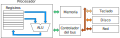
\includegraphics[scale=1]{img/sistema.pdf} \end{center}
    % \textcolor{naranjauca}{Hasta el momento, un bus era un camino eléctrico entre varios dispositivos.}\\
    \begin{center}
    \textcolor{verdeuca}{Necesitamos \textbf{conectar} dispositivos con el procesador.}
    \end{center}
    \pause
    \vspace{-0.3cm}
    \begin{block}{\Large Bus}
    Canal encargado de transferir datos entre componentes o dispositivos. 
    Se compone por un conjunto de cables o líneas que se utilizan respetando un protocolo de control.
    \end{block}
\end{frame}

\begin{frame}[fragile]{Buses}
    Los buses nos permiten conectar dispositivos entre sí.\\
    \bigskip
    Clasifican sus señales en tres tipos básicos:
    \begin{itemize}
    \item \textbf{Direcciones}: Conjunto de señales que conforman la dirección a leer o escribir.
    \item \textbf{Datos}: Conjunto de señales donde se escriben los datos a operar.
    \item \textbf{Control}: Señales que identifican la operación a realizar -lectura o escritura- y sus características.
    \end{itemize}
    \pause
    Para que múltiples dispositivos puedan usar estas líneas,\\ estos deben respetar un \textbf{protocolo de bus}.\\
    \bigskip
    El protocolo describe el conjunto de reglas para:
    \begin{itemize}
    \item Iniciar y realizar una operación sobre el bus (\textbf{master}).
    \item Detectar cuándo se debe responder a un pedido del bus (\textbf{slave}).
    \end{itemize}
    % --CLASE-- ejemplo: master CPU y slave Memoria.
\end{frame}

\begin{frame}[fragile]{Tipos de buses}
    Los \textcolor{naranjauca}{protocolos} los podemos clasificar en:
    \begin{itemize}
    \item \textbf{Sincrónicos}: Existe una señal distinguida (clock) que sincroniza todas las etapas del protocolo del bus.
    \item \textbf{Asincrónicos}: No existe ninguna señal que marque el tiempo. El protocolo opera identificando cambios de estado de las señales.
    \end{itemize}
    \bigskip
    \pause
    Según el uso de las líneas:\\
    \begin{itemize}
    \item \textbf{Dedicadas}: Cada línea tiene un propósito específico.
    \item \textbf{Multiplexadas}: Cada línea varía su uso de acuerdo a en qué etapa se encuentra del protocolo.
    \end{itemize}
    \bigskip
    \pause
    Según el modo de transferencia:\\
    \begin{itemize}
    \item \textbf{Serie}: La información se envía de forma secuencial, bit tras bit.
    \item \textbf{Paralelo}: La información se envía simultáneamente por distintas líneas.
    \end{itemize}
\end{frame}

\begin{frame}[fragile]{Ejemplo protocolos}
    \begin{textblock}{60}(10,15)
    \textbf{Sincrónico}\\ %- Ejemplo lectura de memoria datos lineas mutiplexadas\\
    \only<2->{
    \vspace{0.2cm}
    \includegraphics[scale=0.5]{img/protocolo-layer1.pdf}
    \vspace{0.2cm}
    \scriptsize
    \begin{enumerate}
     \item El \texttt{master} coloca la dirección en el bus, levanta su señal de \texttt{request} y setea la señal de lectura.
     \item El \texttt{slave} levanta la señal de \texttt{ack} hasta que tiene el dato.
     \item El \texttt{slave} baja la señal de \texttt{ack} y al ciclo siguiente presenta el dato durante un clock.
     \item El \texttt{master} baja todas las señales.
    \end{enumerate}
    }
    \end{textblock}
    \begin{textblock}{60}(80,15)
    \textbf{Asincrónico}\\ %- Ejemplo escritura a memoria\\
    \only<3->{
    \vspace{0.2cm}
    \includegraphics[scale=0.5]{img/protocolo-layer2.pdf}
    \vspace{0.2cm}
    \scriptsize
    \begin{enumerate}
     \item El \texttt{master} coloca la dirección en el bus, levanta su señal de \texttt{request} y setea la señal de lectura.
     \item El \texttt{slave} escucha la señal de \texttt{request}, comienza la lecuta y levanta la señal de \texttt{ack}.
     \item El \texttt{slave} presenta el dato leído y baja la señal de \texttt{ack}.
     \item El \texttt{master} lee el dato y baja la señal de \texttt{request}.
    \end{enumerate}
    }
    \end{textblock}
\end{frame}

\begin{frame}[fragile,t]{Árbitro del bus}
    Cuando sobre un bus existen múltiples dispositivos que pueden inciar una operación,\\
    es decir, actuar como \textbf{master}, se debe arbitrar el uso del mismo.\\
    \begin{textblock}{65}(10,27)
    \only<2->{
     \textbf{Árbitro centralizado}\\
     \small Existe un dispositivo denominado árbitro, que recibe todas las señales de solicitud del bus y decide a qué dispositivo le otorga el uso.
     }
    \end{textblock}
    \begin{textblock}{65}(10,55)
    \only<3->{
     \textbf{Árbitro descentralizado}\\
     \small Cada dispositivo recibe información parcial de las solicitudes de uso del bus y cada uno decide independiente y de forma determinística a qué dispositivo se le otorga el bus.
     }
    \end{textblock}
    \begin{textblock}{70}(80,27)
     \only<2->{\includegraphics[scale=0.7]{img/arbitro-layer1.pdf}}
    \end{textblock}
    \begin{textblock}{70}(80,55)
     \only<3->{\includegraphics[scale=0.7]{img/arbitro-layer2.pdf}}
    \end{textblock}
\end{frame}

% \begin{frame}[fragile]{Ejemplos de buses}
%  \begin{itemize}
%     \item PCI
%     %  INSERTAR DIBUJO EJEMPLO
%     \item USB
%     %  INSERTAR DIBUJO EJEMPLO
%     \item IO Bus
%     %  INSERTAR DIBUJO EJEMPLO
% \end{itemize}
% \end{frame}

\begin{frame}[fragile,t]{Interfaz de Entrada-Salida}
    Exiten dos formas básicas de acceder a dispositivos de E/S:
    \begin{textblock}{70}(10,27)
    \only<2->{
    \textbf{Bus de E/S independiente}\\ \small
    El procesador cuenta con un bus especial para acceder a un espacio de entrada-salida.\\
    Se suelen utilizar instrucciones específicas para acceder a este espacio (\texttt{in} y \texttt{out}).
    }
    \end{textblock}
    \begin{textblock}{70}(10,55)
    \only<3->{
    \textbf{Espacio de E/S mapeado a memoria}\\ \small
    El controlador del bus se ocupa de decodificar las direcciones y dependiendo del rango, se accede a la memoria principal o a memoria de un dispositivo.
    Se accede al espacio de la misma forma que una lectura o escritura a memoria.
    }
    \end{textblock}
    \begin{textblock}{70}(89,27)
     \only<2->{\includegraphics[scale=1]{img/lineasDeBus-layer1.pdf}}
    \end{textblock}
    \begin{textblock}{70}(89,55)
     \only<3->{\includegraphics[scale=1]{img/lineasDeBus-layer2.pdf}}
    \end{textblock}
\end{frame}

\begin{frame}[fragile]{Ejemplos de Entrada-Salida}
    \begin{textblock}{60}(10,15)
    \only<2->{
    \textcolor{gray}{\textbf{Ejemplo:} Mapeado a memoria}\\ Memoria de video.\\
    \vspace{0.4cm}
     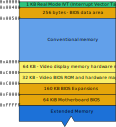
\includegraphics[scale=0.4]{img/memoriaVideo.pdf} 
     }
    \end{textblock}
    \begin{textblock}{60}(80,15)
    \only<3->{
    \textcolor{gray}{\textbf{Ejemplo:} Espacio de E/S}\\ Dispositivo controlador de teclado.\\
    \vspace{0.4cm}
     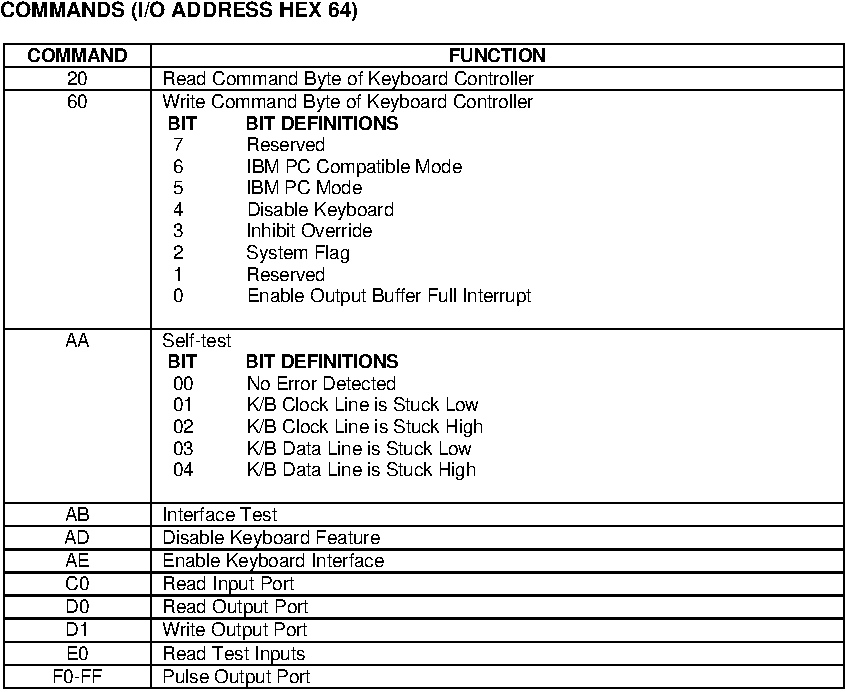
\includegraphics[scale=0.45]{img/interruptController.pdf}
     }
    \end{textblock}
\end{frame}

\begin{frame}[fragile]{Eventos de Entrada-Salida}
    Además de interactuar, realizando lecturas y escrituras sobre el dispositivo de E/S,\\
    debemos poder detectar \textbf{eventos} que le suceden a los dispositivos de E/S.
    \bigskip
    \begin{itemize}
    \setlength\itemsep{0.5cm}
    \item<1-> \textbf{Espera activa}\\
    Se consulta todo el tiempo el estado de los datos y se realiza una acción en base al cambio de estados
    \textcolor{gray}{(Ej. Capturadora de sonido)}.
    \item<2-> \textbf{Interrupciones}\\
    El procesador se detiene, guarda el estado de actual y comienza a ejecutar la rutina que atenderá el pedido
    \textcolor{gray}{(Ej. Teclado)}.
    \item<3-> \textbf{Acceso directo a memoria (DMA)}\\
    Se configura un dispositivo especial, que actúa como master en el bus y permite copiar datos entre diferentes dispositivos
    \textcolor{gray}{(Ej. Copia de bloques en el disco rígido)}.
    \end{itemize}
\end{frame}

\begin{frame}[fragile]{Ejemplos de Entrada-Salida}
    \small
    Suponer un sistema conectado a una capturadora de datos.
    La capturadora tiene dos registros: uno que indica el número de muestra (\texttt{counter}) y otro que indica el valor de la muestra (\texttt{value}).
    Estos están expuestos en direcciones de memoria.
    \begin{itemize}
    \item<2-> \textbf{Espera activa}\\
    \begin{verbatim}
    current = 0
    main:
        while(true):
            if current != counter:
                guardarMuestra(counter, value)
                current = counter
    \end{verbatim}
    \item<3-> \textbf{Interrupciones}\\
    \begin{verbatim}
    int:
        guardarMuestra(counter, value)
        iret
    \end{verbatim}
    \end{itemize}
\end{frame}

\begin{frame}[fragile]{DMA (direct memory access)}
    \begin{textblock}{75}(10,15)
    El \textcolor{naranjauca}{DMA} es un dispositivo programable que actúa como \texttt{master} del bus en remplazo de la \texttt{CPU}.\\
    \bigskip
    \uncover<2->{\textcolor{verdeuca}{La idea es que la CPU pueda seguir procesando mientras el DMA se ocupa de la copia de datos.}\\}
    \bigskip
    \uncover<3->{La CPU configura al DMA para copiar datos entre los dispositivos y la memoria.\\}
    \bigskip
    \small
    \uncover<4->{La configuración de un DMA consiste en:
    \begin{itemize}
    \setlength\itemsep{0cm}
     \item \texttt{address}: Dirección de comienzo del bloque de memoria a copiar.
     \item \texttt{size}: Cantidad de bytes a procesar.
     \item \texttt{device}: Identificador del dispositivo.
     \item \texttt{action}: Leer o escribir.
    \end{itemize}
    }
    \end{textblock}
    \begin{textblock}{70}(90,20)
     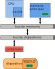
\includegraphics[scale=0.7]{img/dma.pdf}
    \end{textblock}
\end{frame}

\begin{frame}[fragile,t]{Controlador de interrupciones}
    Los sistemas pueden contar con una o múltiples entradas de interrupciones.\\
    \begin{textblock}{70}(10,25)
    \uncover<2->{Si quisieramos tener más interrupciones, contamos con un componente nuevo:\\ el \textcolor{naranjauca}{controlador de interrupciones}.\\}
    \end{textblock}
    \begin{textblock}{70}(75,20)
     \uncover<2->{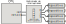
\includegraphics[scale=1]{img/controladorDeInterrupciones.pdf}}
    \end{textblock}
    \vspace{3cm}
    \uncover<3->{
    Este dispositivo se ocupa de:\\
    \begin{itemize}
    \item Determinar qué interrupción se produjo teniendo en cuenta su \textbf{prioridad}.
    \item Establecer el \textbf{vector de interrupciones}, indicando el número de interrupción producida.
    \item Validar si las interrupciones deben ser atendidas en base a la \textbf{máscara de interrupciones}.
    \end{itemize}
    }
    \vspace{0.5cm}
    \uncover<4->{
    \textcolor{verdeuca}{La señal \texttt{INT-ACK} es producida por el procesador y le indica al controlador de interrupciones cuando una interrupción fue atendida.}
    }
\end{frame}

\begin{frame}[fragile,t]{Relación de las interrupciones con el ciclo de instrucción}
    Las interrupciones \textbf{no se pueden atender instantáneamente} cuando llegan ya que no es posible ejecutar la mitad de una instrucción.
    Esto determina que el procesador decide cuándo comprobar si existen interrupciones y cuándo estas serán atendidas.\
    En general, este proceso ocurre previo al \emph{fetch} de la instrucción.\\
    \begin{textblock}{70}(36,36) \only<1->{\includegraphics[scale=0.85]{img/fetchDecodeExecuteWithInt-layer1.pdf}} \end{textblock}
    \begin{textblock}{70}(36,36) \only<2->{\includegraphics[scale=0.85]{img/fetchDecodeExecuteWithInt-layer2.pdf}} \end{textblock}
    \begin{textblock}{70}(36,36) \only<3->{\includegraphics[scale=0.85]{img/fetchDecodeExecuteWithInt-layer3.pdf}} \end{textblock}
    \begin{textblock}{70}(36,36) \only<4->{\includegraphics[scale=0.85]{img/fetchDecodeExecuteWithInt-layer4.pdf}} \end{textblock}
\end{frame}

\begin{frame}[fragile]{Tipos de interrupciones}
    Dependiendo de la fuente de generación de las interrupciones, las podemos clasificar en:
    \bigskip
    \begin{itemize}
    \setlength\itemsep{0.5cm}
    \item<2-> \normalsize \textbf{Interrupciones externas}:
    \small Son producidas por dispositivos externos y llegan al procesador mediante una señal enviada por el controlador de interrupciones \textcolor{gray}{(Ej: teclado)}.
    \item<3-> \normalsize \textbf{Interrupciones sincrónicas}:
    \small Son generadas mediante instrucciones que cambian el flujo del programa. Generalmente se utilizan para modelar servicios del sistema operativo.
    Dependiendo del procesador, se puede utilizar un mecanismo de interrupciones o instrucciones específicas para llamar a servicios del sistema. \textcolor{gray}{(Ej: \texttt{int 0x80})}.
    \item<4-> \normalsize \textbf{Excepciones}:
    \small Es un tipo especial de interrupción que se da cuando el procesador genera un error. La interrupción detiene el programa, ejecutando código que permite entender qué sucedió y arreglarlo
    \textcolor{gray}{(Ej: Intentar ejecutar una instrucción inválida o ejecutar una división por cero)}.\\
    \footnotesize
    Cuando se produce un error, se pueden dar tres casos:\\
     \begin{itemize}
      \item \textit{volver a ejecutar la instrucción que produjo el error luego de arreglarlo} (\textbf{fault})
      \item \textit{ejecutar la próxima instrucción porque nada se puede hacer} (\textbf{trap})
      \item \textit{no se puede conocer exactamente dónde se produjo el error} (\textbf{abort})
     \end{itemize}
    \end{itemize}
\end{frame}

\begin{frame}[fragile,t]{Rutinas de atención de interrupciones}
    Las rutinas de atención de interrupciones son ejecutadas por el procesador cuando una interrupción es generada.
    El procesador guarda una \textbf{tabla} con la dirección donde comienza cada una de las rutinas de atención de interrupciones para cada interrupción posible.\\
    \begin{textblock}{50}(10,30)
    Una rutina de atención de interrupciones tipo tiene la siguiente estructura:
    \end{textblock}
    \begin{textblock}{70}(70,30) \only<1->{\includegraphics[scale=0.85]{img/rutinaInterrupciones-layer1.pdf}} \end{textblock}
    \begin{textblock}{70}(70,30) \only<2->{\includegraphics[scale=0.85]{img/rutinaInterrupciones-layer2.pdf}} \end{textblock}
    \begin{textblock}{70}(70,30) \only<3->{\includegraphics[scale=0.85]{img/rutinaInterrupciones-layer3.pdf}} \end{textblock}
    \begin{textblock}{70}(70,30) \only<4->{\includegraphics[scale=0.85]{img/rutinaInterrupciones-layer4.pdf}} \end{textblock}
    \begin{textblock}{70}(70,30) \only<5->{\includegraphics[scale=0.85]{img/rutinaInterrupciones-layer5.pdf}} \end{textblock}
    \begin{textblock}{70}(70,30) \only<6->{\includegraphics[scale=0.85]{img/rutinaInterrupciones-layer6.pdf}} \end{textblock}
    \begin{textblock}{70}(70,30) \only<7->{\includegraphics[scale=0.85]{img/rutinaInterrupciones-layer7.pdf}} \end{textblock}
    \begin{textblock}{50}(10,50)
    \uncover<2->{\textcolor{verdeuca}{
    El identificador de la interrupción se usa como \textbf{índice} para encontrar el código de la rutina a ejecutar.
    }}
    \end{textblock}
\end{frame}

\begin{frame}[fragile,t]{Ejemplo: ``Teclado númerico''}
    \begin{textblock}{60}(10,15)
    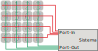
\includegraphics[scale=0.5]{img/tecladoNumerico.pdf}\\
    \end{textblock}
    \begin{textblock}{80}(70,5)
    \small Se tienen dos puertos \texttt{portIn} y \texttt{portOut}
    conectados a un teclado. Ambos mapeados a memoria. Cualquier cambio en \texttt{portIn} genera una interrupción.
    Se desea agregar a un \texttt{buffer} las teclas presionadas.
    \end{textblock}
    \begin{textblock}{100}(5,49)
    \textcolor{naranjauca}{Rutina principal}
    \small
    \vspace{-0.2cm}
    \begin{verbatim}
    main:
        while(true)
            MEM[portOut] = 0x1
            MEM[portOut] = 0x2
            MEM[portOut] = 0x4
            MEM[portOut] = 0x8
    \end{verbatim}
    \end{textblock}        
    \begin{textblock}{100}(70,26)
    \textcolor{naranjauca}{Rutina de atención de interrupciones}
    \small
    \vspace{-0.2cm}
    \begin{verbatim}
    int:
        horizotal = MEM[portIn]
        vertical = MEM[portOut]
        if( horizotal == 1 ) value = 0
        if( horizotal == 2 ) value = 1
        if( horizotal == 4 ) value = 2
        if( horizotal == 8 ) value = 3
        if( vertical == 1 ) value += 0
        if( vertical == 2 ) value += 4
        if( vertical == 4 ) value += 8
        if( vertical == 8 ) value += 12
        addBuffer(value)
        iret
    \end{verbatim}
    \end{textblock}
\end{frame}

\begin{frame}[fragile,t]{Ejemplo: ``Cinta trasportadora''}
    \begin{textblock}{60}(5,15)
    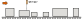
\includegraphics[scale=0.7]{img/cintaTransportadora.pdf}\\
    \end{textblock}
    \begin{textblock}{80}(70,5)
    \small Se tiene un sensor que detecta la presencia de un objeto. Reporta \texttt{0xFF} si hay un objeto y \texttt{0} en caso contrario.
    El sensor se encuentra mapeado a memoria. Se desea contar la cantidad de objetos que son detectados por el sensor.
    \end{textblock}
    \begin{textblock}{100}(15,40)
    \textcolor{naranjauca}{Rutina principal}
    \small
    \vspace{-0.2cm}
    \begin{verbatim}
    contador = 0
    anterior = 0
        main:
            while(true):
                if( anterior != sensor )
                    if( sensor == 0xFF )
                        contador = contador + 1
                    anterior = sensor
    \end{verbatim}
    \end{textblock}
\end{frame}

% \begin{frame}[fragile,t]{Ejemplo: ``Escribir en disco''}
% FIGURA
% \end{frame}

\begin{frame}[fragile]
    \frametitle{Bibliografía}
    \begin{itemize}
     \setlength\itemsep{0.5cm}
    \item[-] \small Tanenbaum, “Organización de Computadoras. Un Enfoque Estructurado”, 4ta Edición, 2000.\\
    \begin{itemize}
     \item \textbf{Selecccionados}\\
     \begin{itemize}
      \item 2.4 Entrada/Salida - Páginas 89 - 92
      \item 3.4 Chips de CPU y buses - Páginas 154 - 170
      \item 3.7 Interfaces - Páginas 193 - 197
      \item 5.5.7 Entrada/Salida - Páginas 356 - 359
      \item 5.6.4 Trampas - Página 379
      \item 5.6.5 Interrupciones - Páginas 379 - 383
     \end{itemize}
    \end{itemize}
    \item[-] \small Null, “Essentials of Computer Organization and Architecture”, 5th Edition, 2018.\\
    \begin{itemize}
    \item \textbf{Chapter 7 - Input/Output Systems}    
     \begin{itemize}
        \item 7.4 I/O Architectures
        \item 7.4.1 I/O Control Methods
        \item 7.4.3 I/O Bus Operation
     \end{itemize}
    \end{itemize}
%     \item[-] \small Silberschatz, “Fundamentos de Sistemas Operativos”, 7ma Edición, 2006.\\
%     \item[-] \small Tanenbaum, “Modern Operating Systems”, 4th Edition, 2015.\\
    \end{itemize}
\end{frame}

\begin{frame}[fragile]
    \frametitle{Ejercicios}
    Con lo visto, ya pueden resolver todos los ejercicios de la guía de ejercicio número 5.
\end{frame}

\begin{frame}[plain]
    \begin{center}
    \vspace{2cm}
    \huge ¡Gracias!\\
    \vspace{2cm}
    \normalsize Recuerden leer los comentarios adjuntos\\ en cada clase por aclaraciones.
    \end{center}
\end{frame}

\end{document}

% % % % % % % % % % % % % % % % % % 
% EJEMPLOS:

\begin{frame}[fragile]
    \frametitle{Bla}
    \begin{itemize}
    \item[-] Bla bla \textbf{ble} bla bla
    \item[-] Bla bla \textbf{ble} bla bla
    \end{itemize}
\end{frame}

\begin{frame}[fragile]
    \frametitle{Bla}
    \begin{block}{\texttt{BLA}}
    Bla Bla
    \end{block}
    \begin{multicols}{2}
    \begin{tabular}{ll}
    la & la \\
    \end{tabular}
    \columnbreak
    \begin{tabular}{ll}
    la & la \\
    \end{tabular}
    \end{multicols}
\end{frame}

\begin{frame}
    \frametitle{Bla}
    \begin{itemize}
    \item Bla bla
    \begin{center}
    \includegraphics[scale=0.7]{img/struct_aling.pdf}
    \end{center}
    Bla bla
    \end{itemize}
\end{frame}

\begin{frame}[fragile]
    \frametitle{Bla}
    \begin{textblock}{100}(10,10)
    Bla
    \end{textblock}
\end{frame}

\end{document}

